\chapter{Consideraciones del Modelo de PHOEBE}

El resultado final obtenido en el
\refthesischapter{metodologia:modelocomputacional} está sujeto a varias
consideraciones. En general, es imposible constreñir de manera adecuada varios
parámetros del modelo de un sistema binario estelar utilizando solo curvas
fotométricas resueltas en el tiempo, y aún menos con solo magnitudes
diferenciales. Para tener un modelo más completo se requiere datos
complementarios, como curvas de velocidades radiales para poder obtener el
semi-eje mayor en unidades reales y por ende las masas de ambas
componentes\textemdash cosa que es posible dentro de PHOEBE utilizando
estimadores y optimizadores adicionales a los empleados en este proyecto de
investigación. En este capítulo se plasman detalles particulares con el modelo
sintético derivado, incluyendo degeneraciones en el modelo y un comportamiento
multi-modal que considerar.

\section{Datos Espectroscópicos}

En el transcurso de este proyecto se buscó entre otras fuentes adicionales para
intentar encontrar observaciones espectroscópicas de \atoObjId que pudieran
constreñir otros parámetros del sistema, como la temperatura efectiva del
sistema (la cual se dejaría como parámetro fijo en vez de utilizar la diferencia
de color en el flujo de ZTF) o la masa de la estrella primaria, la cual no se
puede constreñir utilizando solo curvas de luz fotométricas. A pesar de las
capacidades avanzadas de PHOEBE, actualmente no tiene manera de generar un
espectro sintético con cual comparar a un espectro observado. En total se
obtuvieron 3 espectros independientes de \atoObjIdNoSpace : 2 de ellos fueron
proporcionados por la Dra. Paula Szkody de la Universidad de Washington, y 1
espectro obtenido del catálogo Gaia DR3.

\subsection{Apache Point Observatory}

Desde el \textit{Observatorio Apache Point} (\textit{Apache Point Observatory})
la Dra. Szkody logró observar a \atoObjId con el telescopio \textbf{ARC 3.5m}
con el espectrógrafo \textbf{KOSMOS}, un espectrógrafo de baja resolución ($R
\sim 2200$) con una rendija de 0.86 pulgadas en la posición \textit{Alta}, la
cual resulta en un rango de longitudes de onda de $4150 - 7050 \Angstrom$. La
información técnica de KOSMOS se encuentra en la documentación en línea de
KOSMOS\footnote{\url{https://www.apo.nmsu.edu/arc35m/Instruments/KOSMOS/userguide.html}}.
Ambos espectros se pueden ver en la \reffigure{figuraEspectrosApo}.

\begin{figure}[!ht]
    \centering
    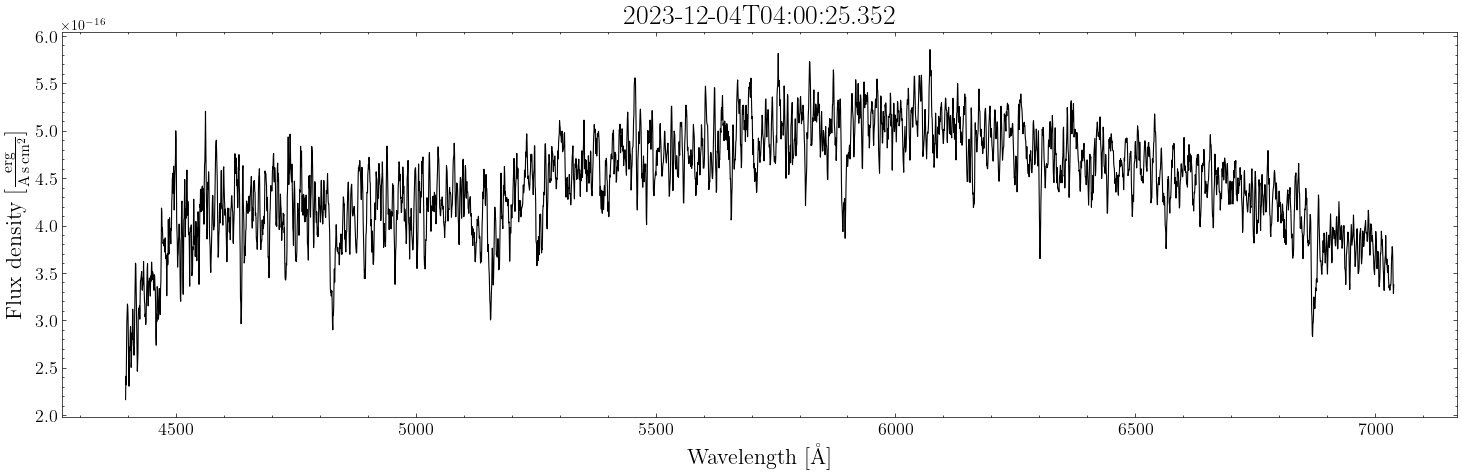
\includegraphics[scale=0.45]{Conclusion/Figures/Figura APO Spectrum 2.png}
    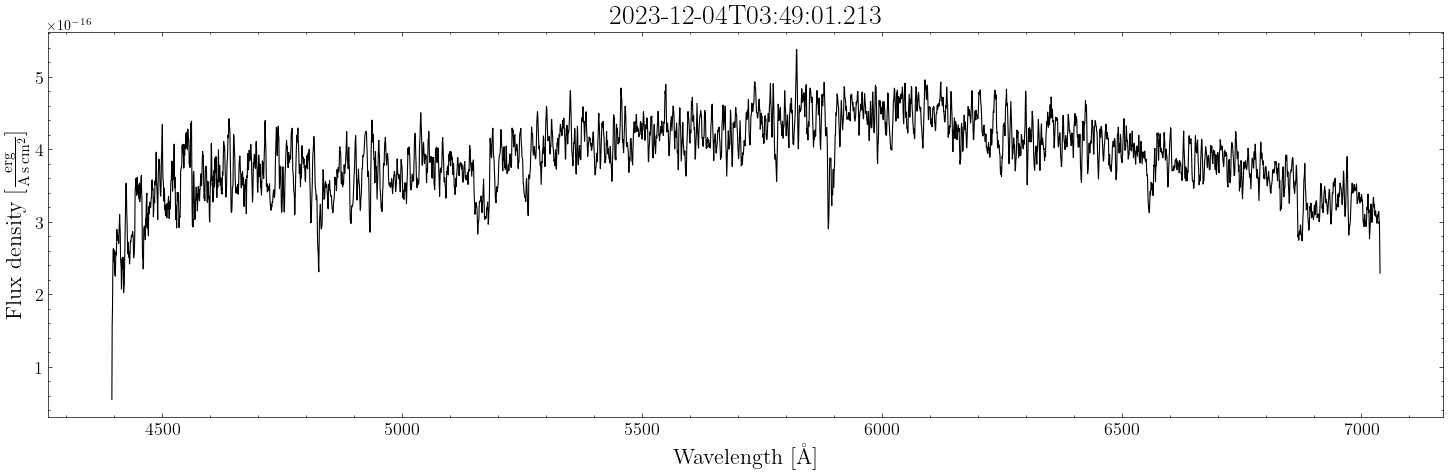
\includegraphics[scale=0.45]{Conclusion/Figures/Figura APO Spectrum 1.png}
    \caption{Espectros tomados de \atoObjId por la Dra. Paula Szkody desde APO.}
    \label{figuraEspectrosApo}
\end{figure}

Los espectros de KOSMOS fueron tomados la misma noche del 4 de diciembre del
2023 en exposiciones de 10 minutos consecutivas. Sin embargo, ambos espectros
muestran una baja razón de señal a ruido (SNR), probablemente por el bajo tiempo
de exposición. Para aumentar el SNR se generó un espectro promedio entre los dos
espectros individuales. Utilizando la función \code{snr\_derived} del paquete
\code{specutils}\footnote{\url{https://specutils.readthedocs.io/en/stable/index.html}}
es posible estimar el SNR basado en solo el espectro medido del archivo. La
función \code{snr\_derived} implementa un algoritmo general para esta tarea,
donde se considera que la señal principal cae en un continuo; el ruido se mide
por la dispersión alrededor del medio del espectro. El espectro promedio se
puede ver en la \reffigure{figuraEspectroApoPromedio}, para el cual el SNR
calculado es de 50.94, a comparación de 39.54 y 38.98 respectivamente de los
espectros individuales en la \reffigure{figuraEspectrosApo}.

\begin{figure}[!ht]
    \centering
    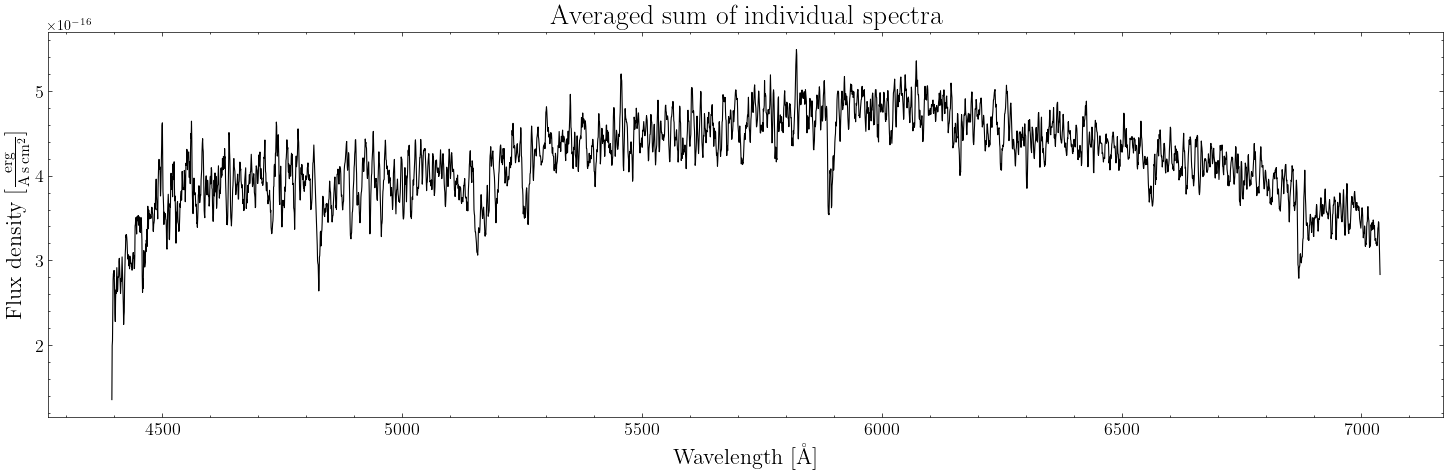
\includegraphics[scale=0.45]{Conclusion/Figures/Figura APO Spectrum Average.png}
    \caption{Espectro promedio de \atoObjIdNoSpace, utilizando el flujo promedio en cada longitud de onda de ambos espectros en la \reffigure{figuraEspectrosApo}.}
    \label{figuraEspectroApoPromedio}
\end{figure}

\subsection{Gaia DR3}

Junto a las curvas de luz fotométricas descritas en la
\refthesissection{muestra:gaia} Gaia DR3 ofrece espectros de aproximadamente 220
millones de las fuentes observadas. Gaia cuenta con un arreglo de
espectro-fotómetros BP y RP (los cuales corresponden a las pasabandas
\textit{Gaia:BP} y \textit{Gaia:RP} respectivamente) que cubren los rangos $[330
- 680] \ \mathrm{nm}$ para BP y $[640 - 1050] \ \mathrm{nm}$ para RP
[\citeyearparen{carrasco_internal_calibration_gdr3_bprp_low_resolution_spectra_2021}].
Cada transito de un objeto por el campo de visión de Gaia contribuye al espectro
promedio de baja resolución; la resolución espectral varía con la longitud de
onda observada, yendo de 100 a 30 para el rango espectral de BP y de 100 a 70
para RP (visto en la figura 3 de
\citeyearparen{carrasco_internal_calibration_gdr3_bprp_low_resolution_spectra_2021}).
Es posible determinar si una fuente en Gaia DR3 cuenta con un espectro por medio
del campo \code{has\_xp\_continuous}. Integrando el espectro en cada rango de
longitud de onda se obtiene el flujo total en Gaia:BP y Gaia:RP.

Para obtener datos limpios de calidad adecuada se someten a un proceso de
calibración extenso, incluyendo la distorsión por la geometría del CCD y la
caracterización del espacio local del objeto\textemdash una revisión extensa del
procesamiento y validación es dada por
\citeyearparen{de_angeli_gdr3_processing_and_validation_bprp_spectra_2023}. El
espectro observado $h_{s,k}(u_i)$ dado un sistema de pseudo-longitudes de onda
$u$ en el catálogo Gaia DR3 se da como una combinación lineal de una función de
base $\varphi$ para una fuente $s$:

\begin{eqfloat}[!ht]
    \begin{equation}
        h_{s,k}(u_i) = \sum_{n=0}^{N - 1} b_{s,n} \sum_{j = -J}^{J} A_k(u_i, u_{i+j}) \varphi_n(u_i+j)
    \end{equation}
\end{eqfloat}

Donde $k$ denota una unidad de calibración (un intervalo de parámetros continuos
cuya variación es baja
[\citeyearparen{carrasco_internal_calibration_gdr3_bprp_low_resolution_spectra_2021}]),
$b_s$ son los coeficientes que contienen la información necesaria para construir
el espectro BP/RP de la fuente, y $A_k$ es el modelo del instrumento. La función
de base elegida por su ortogonalidad, su convergencia a 0 dado un valor de
entrada suficientemente alto, y su centro en $\theta = 0$ se utilizaron
funciones Hermite como las bases del espectro continuo:

\begin{eqfloat}
    \centering
    \begin{equation}
        \begin{split}
            & \varphi_0(\theta) = \pi^{-\frac{1}{4}} e^{-\frac{\theta^2}{2}} \\
            & \varphi_1(\theta) = \sqrt{2} \pi^{-\frac{1}{4}} \theta e^{-\frac{\theta^2}{2}} \\
            & \varphi_n(\theta) = \sqrt{\frac{2}{n}} \theta \varphi_{n-1}(\theta) - \sqrt{\frac{n - 1}{n}} \varphi_{n-2}(\theta)
        \end{split}
    \end{equation}
\end{eqfloat}

Donde se define la transformación lineal de las pseudo-longitudes de onda
$\theta = \Theta \cdot u + \Delta \theta$ con el factor de escala $\Theta$ y un
desplazamiento de $\Delta \theta$ basado en el espectro de la fuente $s$. El
archivo disponible a través del servicio DataLink de Gaia DR3 contiene los
coeficientes de las funciones de base para los espectros BP/RP de
\atoObjIdNoSpace, incluyendo los coeficientes de los errores y la matriz de
correlación entre los coeficientes de las funciones de base. Para facilitar la
lectura y el análisis de este espectro el equipo de Gaia ofrece la herramienta
GaiaXPy\footnote{\url{https://gaiaxpy.readthedocs.io/en/latest/index.html}} que
acepta como entrada el archivo del espectro continuo. Utilizando la función
\code{calibrate} de GaiaXPy este se puede muestrear dado una malla de longitudes
de onda reales en unidades $[\mathrm{nm}]$, dando como resultado el espectro
visto en la \reffigure{figuraEspectroGdr3}.

\begin{figure}[!ht]
    \centering
    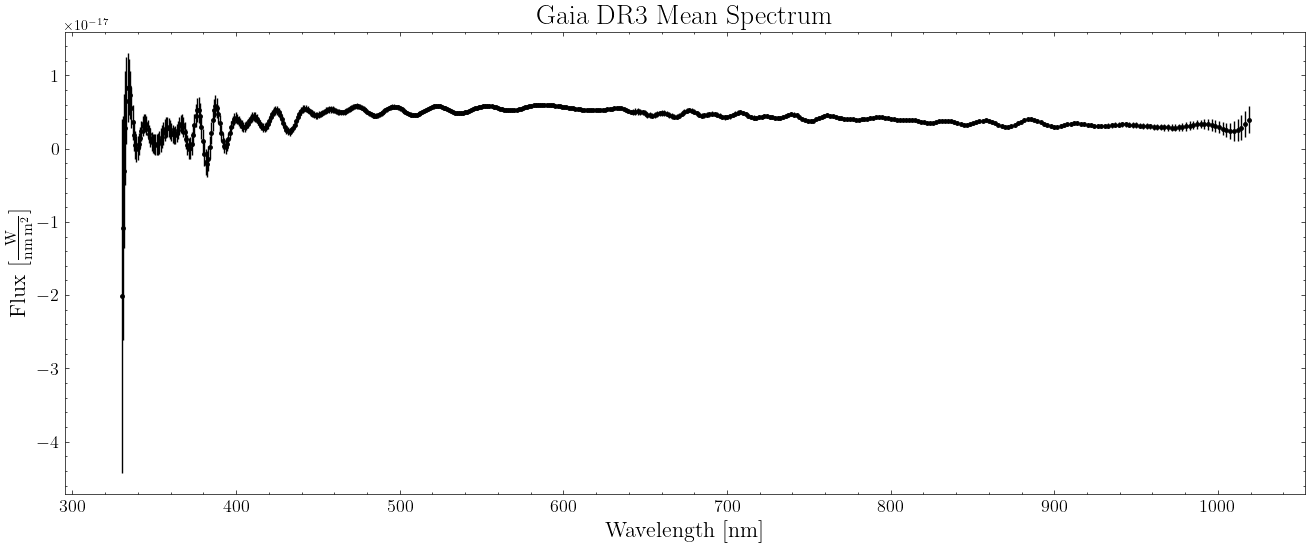
\includegraphics[scale=0.45]{Conclusion/Figures/Figura Gaia DR3 Espectro.png}
    \caption{Espectro continuo de \atoObjId obtenido de Gaia DR3 muestreado
    utilizando una malla de longitudes de onda equidistantes en un espacio
    logarítmico para mejorar la resolución del muestreo en el rango más azul.}
    \label{figuraEspectroGdr3}
\end{figure}

\subsection{Análisis: PyHammer}

Para llevar a cabo un análisis rápido de ambos espectros obtenidos se utilizó la
herramienta de clasificación espectral \textbf{PyHammer}\footnote{Disponible en
GitHub: \url{https://github.com/BU-hammerTeam/PyHammer}}. PyHammer\textemdash
descrito por
\citeyearparen{kesseli_pyhammer1_empirical_template_stellar_spectra_classification_2017}
y después por
\citeyearparen{roulston_pyhammer2_classifying_stars_binaries_stellar_templates_2020}
para la versión 2\textemdash fue desarrollado para facilitar la clasificación
automática y manual de espectros estelares de sistemas binarios por medio de
plantillas espectrales para varios tipos de estrellas, desde tipo O hasta tipo L
generados partiendo de datos del catálogo SDSS BOSS (SDSS Baryon Oscillation
Spectroscopic Survey). Aparte del tipo espectral, PyHammer cuenta con plantillas
para determinar la metalicidad y gravedad superficial (la cual se utiliza para
distinguir entre estrellas enanas y gigantes) basado en líneas espectrales de
referencia. 

Utilizamos ambos espectros especificados en esta sección (el espectro promedio
de APO y el espectro muestreado de Gaia DR3 en una malla de longitudes de onda
uniforme en una escala no logarítmica) para corroborar los parámetros obtenidos
del modelo de PHOEBE. Los resultados de ambos análisis de PyHammer se pueden ver
en la \reffigure{figuraAjustePyHammer}. Ambos resultados indican que el sistema
está compuesto de estrellas tipo K, con una metalicidad de $-0.5 \mathrm{dex}$. 

\begin{figure}[!ht]
    \centering
    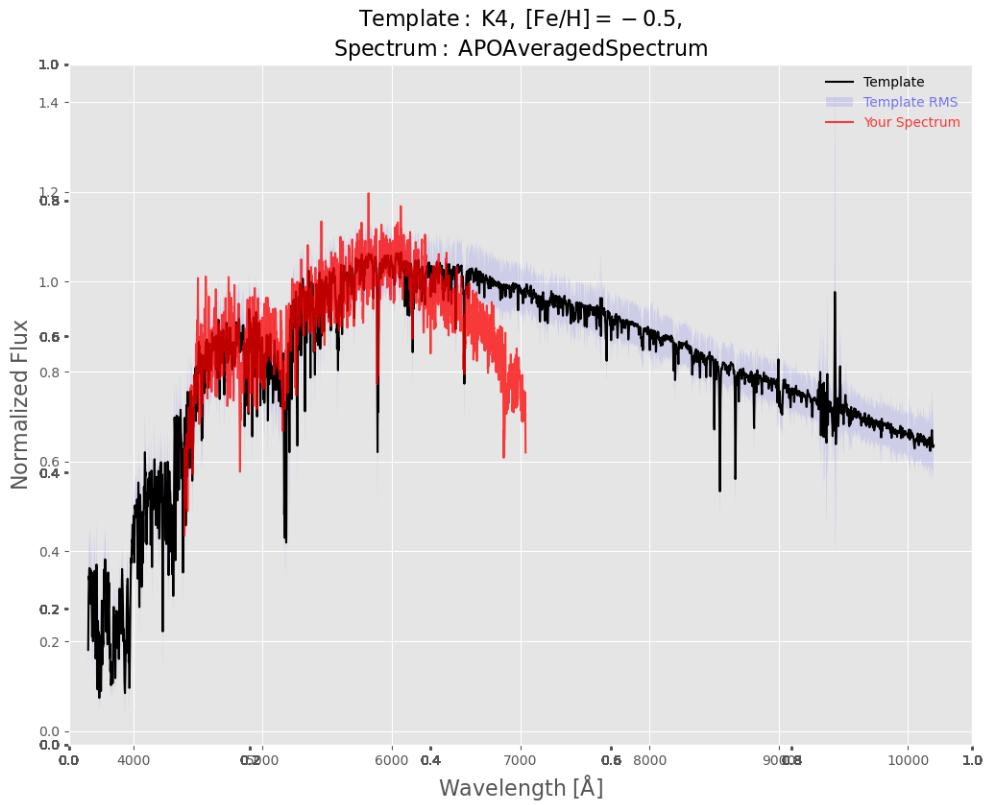
\includegraphics[scale=0.5]{Conclusion/Figures/Figura PyHammer APO.png} \\
    \vspace{0.6em}
    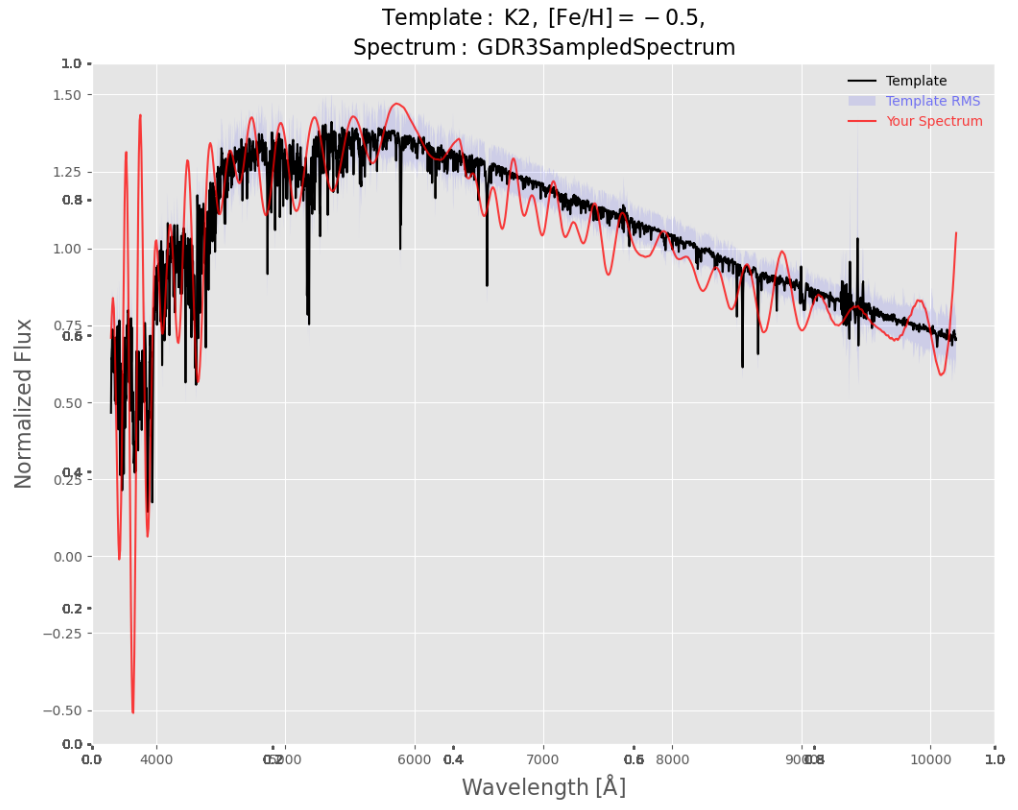
\includegraphics[scale=0.5]{Conclusion/Figures/Figura PyHammer GDR3.png}
    \caption{Resultados del análisis usando PyHammer para el espectro de APO y
    de Gaia DR3 en la gráfica superior e inferior, respectivamente. Partiendo de
    una estimación inicial automática por PyHammer se ajustó el tipo espectral y
    la metalicidad hasta llegar al mejor ajuste visto en esta figura, utilizando
    el $\chi^2$ reportado en la aplicación como guía.}
    \label{figuraAjustePyHammer}
\end{figure}

Los resultados del análisis de PyHammer coinciden con la temperatura efectiva
derivada usando PHOEBE y las curvas fotométricas de ZTF, dado el rango de
temperaturas efectivas de estrellas tipo K de aproximadamente $3900 - 5300
\mathrm{K}$. Sin embargo, mucho cuidado es necesario al interpretar estos
resultados. El espectro de Gaia, a pesar de ser el más completo, es de muy baja
resolución espectral, lo cual causa la perdida de información de las líneas de
emisión y absorción que permitirían una clasificación adecuada del sistema. El
espectro de Gaia también muestra errores significativos en las longitudes de
ondas más cortas, lo cual causa una discrepancia contra el espectro de
plantilla. Al mismo tiempo, el espectro de APO carece de una buena razón de
señal a ruido; a pesar de que la plantilla K4 sea la que mejor se ajusta a los
datos, se puede ver en la gráfica superior de la
\reffigure{figuraAjustePyHammer} un decaimiento repentino en las longitudes de
onda más largas del espectro medido, algo que no se observa en el de Gaia y que
no tenemos una explicación satisfactoria en este trabajo. Dado que la
temperatura efectiva de la componente primaria no tiene un efecto significativo
en la morfología de la curva de luz de un sistema binario en contacto
[\citeyearparen{wadhwa_effective_temperature_light_curve_solutions_cbs_2023}] no
es necesario descartar todo el modelo de PHOEBE para \atoObjIdNoSpace. Un
análisis a mayor profundidad con datos espectroscópicos de mayor precisión
ayudaría a constreñir parámetros adicionales del modelo. En el caso de tener
varios espectros del sistema a lo largo del tiempo se podría construir una curva
de velocidades radiales, la cual se podría ingresar al modelo en PHOEBE
directamente.

\section{Multi-Modalidad de la PDF Posterior}

